\label{chap:03_social_text_classification}

La extracción de opiniones en distintos espacios virtuales ha atraído mucho interés desde los comienzos de la World Wide Web. Inicialmente motivados por fines puramente comerciales, diferentes motivaciones han surgido debido al desarrollo de la técnica y la proliferación de las redes sociales: desde intereses sociológicos (como el análisis de discurso de odio o las reacciones a la pandemia) hasta políticos (como observar cuál es la opinión general sobre tal o cual candidato o sobre un tema candente). Desde principios de los años 2000, y debido a la combinación del desarrollo de métodos de aprendizaje estadístico y la cantidad creciente de datos disponibles generados por usuarios en Internet, numerosos trabajos han analizado este tipo de textos para poder extraer conocimiento \textbf{subjetivo} de estos.

Debido a la inmensa cantidad de contenido generado en diversos sitios y redes sociales (se estima que en el mundo se generan XXX tweets por segundo), hace ya muchos años esta tarea es difícil de realizar sin algún tipo de automatización. Para ello, muchísimo esfuerzo se ha volcado en utilizar técnicas de aprendizaje automático para atacarla. El avance de las técnicas de NLP --como hemos descrito en el capítulo anterior-- han permitido avanzar sobre este terreno; sin embargo, muchas de las limitaciones actuales del área \todo{citar paper Climbing towards NLU} en conjunto a las dificultades particulares de las interacciones en medios sociales hacen esta tarea difícil.

En este capítulo haremos una breve introducción a clasificación de textos sociales. Esto es, dado un texto generado por un usuario (un post en Facebook, Instagram, un tweet, etc) predecir alguna característica discreta de éste, como por ejemplo si es un texto positivo o negativo, si tiene algún tipo de emoción de ira, alegría, u otra; si contiene discurso de odio contra algún grupo o no; si es irónico; entre otras. En base a datasets en español para distintas tareas, presentaremos modelos de clasificación basados en técnicas del estado del arte.

Finalmente, analizaremos algunas cuestiones relacionadas a la adaptación de dominio y representaciones generadas sobre dominios sociales. Analizaremos para técnicas de representación no contextualizadas \footnote{Que al día de la fecha, en pocos años, han quedado obsoletas} y algunas técnicas más recientes el impacto de entrenar desde cero o realizar cierta adaptación sobre la performance de las técnicas de clasificación.


\section{Motivación}

Las motivaciones para extraer opiniones subjetivas de usuarios en Internet son múltiples, aunque intentaremos categorizarlas en algunos grupos de notable interés. Dado el aumento considerable de contenido generado por usuarios desde el comienzo de la WWW --y subsiguientemente con la explosión de las Redes Sociales-- una de las motivaciones es netamente comercial: ¿qué opinan los usuarios sobre este nuevo producto? ¿cuáles creen que son sus falencias? ¿qué tal es el servicio en el Restaurant X? Desde ya más de 20 años, numerosos sitios de e-commerce brindan la posibilidad de que los clientes vuelquen sus opiniones al respecto de los productos que consumen en sus plataformas, como así también pueden incorporarse en otras aplicaciones que brindan esta posibilidad de expresar comentarios sobre productos, servicios u otros lugares. Para citar unos ejemplos, IMDb permite agregar comentarios sobre películas, Google Maps sobre distintos sitios --tanto turísticos como locales comerciales--, o los distintos sitios de venta minorista como MercadoLibre, eBay, o Amazon.

Con la explosión de las redes sociales, otros horizontes de preguntas se abrieron\footnote{Si bien algunas preguntas de carácter sociológico tuvieron lugar con anterioridad, podemos marcar el uso intensivo de Facebook y Twitter como el comienzo de un estudio más sistemático de ellas}. Uno de estos horizontes, que es de interés particular para esta tesis, es el de las preguntas de carácter sociológico. Preguntas que pueden suscitar interés dentro de este punto pueden ser:

\begin{itemize}
    \item ¿cuál es la opinión de los usuarios acerca de la legalización del aborto?
    \item ¿cuál es el sentimiento que tienen ciertos usuarios hacia los inmigrantes subsaharianos en España?
    \item ¿cómo se ha modificado el ``humor social'' de acuerdo a crisis económicas o pandemias como la del COVID-19?
    \item ¿quiénes generan discurso de odio contra la comunidad LGBTI en Argentina?
    \item ¿qué artículos periodísticos suscitan la mayor cantidad de discurso discriminatorio en las redes sociales?
    \item ¿cuáles son las principales preocupaciones de ciertos sectores de la población?
\end{itemize}

entre otras. Estos tópicos son de gran interés para investigadores y políticos. Usualmente, la forma más estandarizada de acceder a la opinión de distintos actores sociales ha sido la de encuestas; sin embargo, la recolección y extracción automática de opiniones de medios virtuales brinda una alternativa (a veces) más económica y masiva aunque con un sesgo poblacional distinto al de otras metodologías.

\todo{Contar algo de Cambridge Analytica?}

\section{Clasificación de textos sociales}

Muchos de estos problemas de extracción de opiniones se pueden plantear como problemas de clasificación\cite{pang2008opinion}: dado un contenido social, queremos predecir una clase $c \in \mathcal{C}$, con $\mathcal{C}$ un conjunto finito de clases. El análisis de polaridad, por ejemplo, se puede plantear como un problema de clasificación en el que dado un texto en una red social, predecir si tiene un sentimiento positivo, negativo, o neutro. El problema de análisis de emociones se puede plantear como, dado un texto, seleccionar la emoción predominante en él de un conjunto de 6 emociones y una neutral.

Algunas variantes de estos problemas se pueden dar en el contenido analizado. Por ejemplo, el \emph{Análisis de Sentimiento basado en aspectos} (usualmente denominada \emph{ABSA} en la literatura por sus siglas en inglés) es una variante de la clasificación de polaridad en la que queremos predecir el sentimiento de un texto para cierto aspecto\cite{pavlopoulos2014aspect}; por ejemplo, en la oración ``lindo lugar, la comida está muy bien pero la cerveza es horrible'' (en una posible reseña de un restaurant) podemos identificar dos sentimientos distintos: uno positivo para la comida y otro negativo para la cerveza.

Dentro de estos problemas que complejizan la entrada, podemos contar algunos de carácter multimodal.  En \citet{sharma-etal-2020-semeval} se plantea un problema de análisis de emociones para memes donde la entrada (el contenido social) consta de imágenes y texto, y se intenta predecir la emoción predominante.

Análogamente, se puede agregar cierta complejidad en la salida. Por ejemplo, el Stanford Sentiment Treebank (SST) \cite{socher-etal-2013-recursive} plantea una tarea de análisis de polaridad asignando una escala de Likert \cite{likert1932technique}: cada comentario está etiquetado como muy negativo, algo negativo, neutral, algo positivo o muy positivo. Así mismo, otra posibilidad es la de predecir conjuntamente varias variables: por ejemplo, predecir si un comentario es discriminatorio, si es dirigido a un grupo o una persona, y si es agresivo, como el dataset de hatEval \cite{hateval2019semeval}; o bien, dado un comentario de una nota periodística, predecir las características que discrimina si es que hay alguna (como ser a las mujeres, al colectivo LGBTI, por motivos raciales, etc). De este último ejemplo hablaremos en los capítulos \ref{chap:05_dataset_creation} y \ref{chap:06_contextualized_hate_speech}.




\section{Trabajo previo}


Dentro de los recursos y tareas en español, uno de los principales polos de esto es el Taller de Análisis de Sentimientos (TASS) \cite{overview_tass2018,garcia2020overview,cumbreras2016overview} organizado por la Sociedad Española de Procesamiento Natural (SEPLN) y en sus últimas dos ediciones (2020 y 2021) organizadas en el marco del evento Iberian Languages Evaluation Forum (IberLEF). En él se presentan tareas y datasets de análisis de sentimiento, de emociones, de toxicidad, sexismo, entre otras. \todo{agregar citas}


\section{Tareas analizadas}

\begin{table}[t]
    \centering
    \begin{tabular}{l ll ll}
        Tarea                     &  Dataset                   & Tamaño         & Clases   &\\
        \mr{3}{Análisis de Sentimientos}  &  \mr{3}{TASS 2020} & \mr{3}{14,509} & Neg      & (39.80\%)\\
                                          &                    &                & Neu      & (29.52\%)\\
                                          &                    &                & Pos      & (30.68\%)\\
        \hline
        \mr{7}{Análisis de emociones}&\mr{7}{TASS 2020/EmoEvent}&\mr{7}{8,409}  & Otra     & (49.08\%)  \\
                                          &                    &                & Alegría  & (21.58\%)  \\
                                          &                    &                & Tristeza & (12.00\%)  \\
                                          &                    &                & Ira      & (10.19\%)  \\
                                          &                    &                & Sorpresa & (4.10\%)  \\
                                          &                    &                & Disgusto & (1.91\%)  \\
                                          &                    &                & Miedo    & (1.14\%)  \\
        \hline
        \mr{2}{Detección de ironía}  & \mr{2}{IroSVa 2019}     & \mr{2}{9,000}  & No irónico   & (66.68\%)\\
                                          &                    &                & Irónico      & (33.32\%)\\
        %Análisis de Emociones     &  TASS 2020/EmoEvent\cite{plaza-del-arco-etal-2020-emoevent} & 7 & 1,879 \\
        \hline
    \end{tabular}
    \caption{Tareas evaluadas en este capítulo, junto a datos estadísticos de los datasets utilizados}
    \label{tab:03_tasks}
\end{table}

Analizamos 3 tareas de extracción de opiniones sobre redes sociales, y las usamos como benchmark para las diferentes técnicas de clasificación. Una de las tareas analizadas es la de \textbf{análisis de polaridad}: dado un tweet, detectar si tiene una polaridad general positiva, negativa, o neutra. Para ello, utilizamos el dataset de TASS 2020\cite{garcia2020overview}, anotados con estas 3 clases y con información de las diferentes variedades dialectales del español a la que pertenece cada tweet. Para nuestro análisis, ignoramos estas distinciones y fusionamos todos los datos en un solo conjunto de datos (con las 3 particiones correspondientes de entrenamiento, validación, y test).


Para el análisis de emociones, también usamos el conjunto de datos de TASS 2020/\emph{EmoEvent} \cite{plaza-del-arco-etal-2020-emoevent}. Este dataset multilingual (español e inglés) contiene tweets etiquetados con las seis emociones básicas de Ekman \cite{ekman1992argument} (\emph {ira}, \emph {disgusto}, \emph {miedo}, \emph {alegría}, \emph {tristeza}, \emph {sorpresa}) y también una emoción ``neutral''. El dataset fue recolectado en base a a ocho eventos globales diferentes de diferentes dominios (políticos, entretenimiento, catástrofes o incidentes, conmemoraciones globales, etc.) por lo que las emociones siempre están relacionadas con un fenómeno en particular. Solo conservamos la parte en español, que contiene 8.409 tweets.


 La \textbf{detección de ironía} también es una tarea que ha ganado popularidad recientemente. Muchos trabajos muestran que tiene importantes implicaciones en otras tareas de procesamiento del lenguaje natural que requieren procesamiento semántico. \citet{gupta-yang-2017-crystalnest} muestran que el uso de funciones derivadas de la detección de sarcasmo mejora el rendimiento en la tarea de análisis de sentimientos. Además de esto, el contenido generado por los usuarios es una rica y vasta fuente de ironía, por lo que esta tarea es de particular importancia para el dominio de las redes sociales. IroSVa \cite {ortega2019overview} es un dataset para esta tarea en Español (publicado en el contexto de TASS 2019) que tiene la particularidad de considerar los mensajes no como textos aislados sino con un contexto dado (un titular o un tema). Consta de 7.200 instancias y 1.800 ejemplos de prueba divididos en tres variantes geográficas de Cuba, España y México, cada una con una etiqueta binaria que indica si el comentario contiene ironía o no. A diferencia de las tres tareas anteriores mencionadas aquí, este conjunto de datos contiene no solo mensajes de Twitter, sino también de comentarios de noticias y foros de debate como 4forums.com y Reddit.

 La tabla \ref{tab:03_tasks} resume los datos de cada uno de los corpus utilizados en este capítulo.


\section{Normalización y preprocesamiento}
\label{sec:03_preprocessing}

Una de los pasos más importantes para la manipulación de texto social es el preprocesamiento. Con esto nos referimos al conjunto de técnicas dedicadas a disminuir la variabilidad del texto y aproximarlo a una forma lo más normal posible \footnote{\citet{eisenstein2013bad} discute siquiera que exista tal forma normal}. El texto generado por usuarios en medios informales suele ser bastante más irregular que el texto proveniente de otras fuentes, con errores ortográficos y usos coloquiales que hacen difícil el tratamiento por algoritmos de NLP. Para poner un ejemplo, la frase ``¡qué lindo día, loco!'' puede ser representada de las siguientes maneras:

\begin{itemize}
    \item q lindo día loco
    \item k lindo diaaaaaaaa loco
    \item ke lendo diaa lk
\end{itemize}

entre otras formas posibles. \citet{han2011lexical} es uno de los primeros trabajos que aborda sistemáticamente este problema para el dominio de redes sociales. En base a un dataset recolectado por los autores, observaron que las palabras fuera de vocabulario (OOV en inglés)\footnote{fuera del vocabulario de un diccionario estándar de GNU en inglés} en Twitter tienen una alta frecuencia de incidencia. Ejemplos de estas palabras son neologismos, errores ortográficos, typos, contracciones típicas de esta red social (lk), sustituciones fonéticas (wacho en vez de guacho), entre otras.Este problema de la desnormalización del texto generado por usuarios plantea un serio inconveniente para los métodos del estado del arte de ese entonces basados en bolsas de palabras o representaciones sobre palabras aisladas \footnote{Recordemos que para el momento de la publicación de este trabajo aún no se usaban redes neuronales, word embeddings, ni mucho menos métodos más avanzados como \emph{fasttext}, que ayuda mucho en las palabras OOV}. Para mitigar el problema de la alta dimensionalidad que generan estas palabras fuera de vocabulario, los autores proponen diversas estrategias para normalizar las palabras y testean sus métodos sobre datasets de Twitter y SMS.

\citet{eisenstein2013bad} trata este problema desde una perspectiva más amplia con los enfoques utilizados hasta el momento. El autor plantea dos posibilidades para las tareas de NLP en el medio social: la \textbf{normalización} sería una forma de adaptar el texto a las herramientas, mientras que la \textbf{adaptación de dominio}\footnote{La definición del autor de dicho trabajo difiere ligeramente de la adaptación de dominio que trataremos en el capítulo \ref{chap:07_domain_adaptation}} sería adaptar las herramientas al texto. Con lo primero nos referimos al conjunto de técnicas que podemos utilizar para acercar la distribución del texto lo más posible a un dominio formal (por ejemplo, sobre el que entrenamos un POS tagger), mientras que por adaptación de dominio nos referimos a la construcción de datasets y algoritmos particulares para distintas tareas de NLP en redes sociales, como por ejemplo POS tagging \cite{gimpel2010part}, NER \cite{ritter2011named}, entre otros.

Con el advenimiento de las redes neuronales y los word-embeddings como GloVe o word2Vec, esto siguió siendo un problema ya que cada representación se calcula sobre cada una de estas palabras. En el caso de una palabra fuera de vocabulario, un mecanismo habitual es asignarles un token especial que se llama ``<unk>''. Sin embargo, esto puede ser problemático ya que elimina muchas palabras similares a otras que sí tenemos en el vocabulario. \citet{bojanowski16} propuso una solución a esto al permitir formar la representación de cada palabra mediante una combinación lineal de las representaciones de las ``subpalabras'' de cada una: cada palabra se separa en una lista de substrings y cada una de estas son los que se calculan los embeddings (ver sección XXX para más detalles).

Con el advenimiento de los modelos basados en transformers, otros tipos de tokenización fueron propuestos que permiten reducir las palabras OOV. BPE \cite{sennrich2016neural}, Word Piece, Sentence Piece \cite{kudo-richardson-2018-sentencepiece} utilizan, en lugar de separar el texto mediante los espacios, en la utilización de distintos tipos de subpalabras. Esta técnica permite reducir la incidencia de palabras OOV notablemente. Ver la sección XXX para más detalles. \todo{citar sección de preliminares}

En el caso de modelos basados en transformers, \citet{bertweet} plantearon experimentos en tareas sociales usando dos formas de normalización: una \textbf{débil}, donde sólo convierten nombres de usuario en un token especial \verb|@USER| y a las urls en otro token especial \verb|HTTPURL|, y otra estrategia \textbf{fuerte} donde usan diccionarios de normalización. Para un conjunto de tareas de clasificación sobre Twitter y distintos modelos pre-entrenados, los resultados de los experimentos arrojaron que la normalización fuerte empeora levemente la performance.

En base a esto, adoptamos una estrategia similar a la normalización \textbf{débil} mencionada en \citet{bertweet}:

\begin{itemize}
    \item  Convertimos los handles se convierte en un token especial \verb|@usuario|
    \item Convertimos URLS en un token especial \verb|URL|
    \item Convertimos los emojis a representaciones textuales usando la librería \emph{emoji} \footnote{\url{https://pypi.org/project/emoji/}}
    \item Normalizamos risas (``jajajajjjjajaja'' lo convertimos a ``jaja'')
    \item Procesamos hashtags: \#EsteHayQueNormalizar lo convertimos a \emph{hashtag esto hay que normalizar}
    \item Limitamos repeticiones de caracteres a 3 ocurrencias
\end{itemize}

Si bien en algunas secciones (como en \ref{sec:04_preprocessing}) usaremos variaciones de estos métodos --particularmente para modelos lineales--, en líneas generales seguiremos esta estrategia de normalización.

\section{Algoritmos de clasificación}

\begin{figure}
    \centering
    % Link a draw
    % https://docs.google.com/drawings/d/1bSCMXkAF12gK4GFYL8tyIAPCMq4kj8JXovrf2lx5w_g/edit
    \begin{subfigure}[t]{\textwidth}
        \centering
        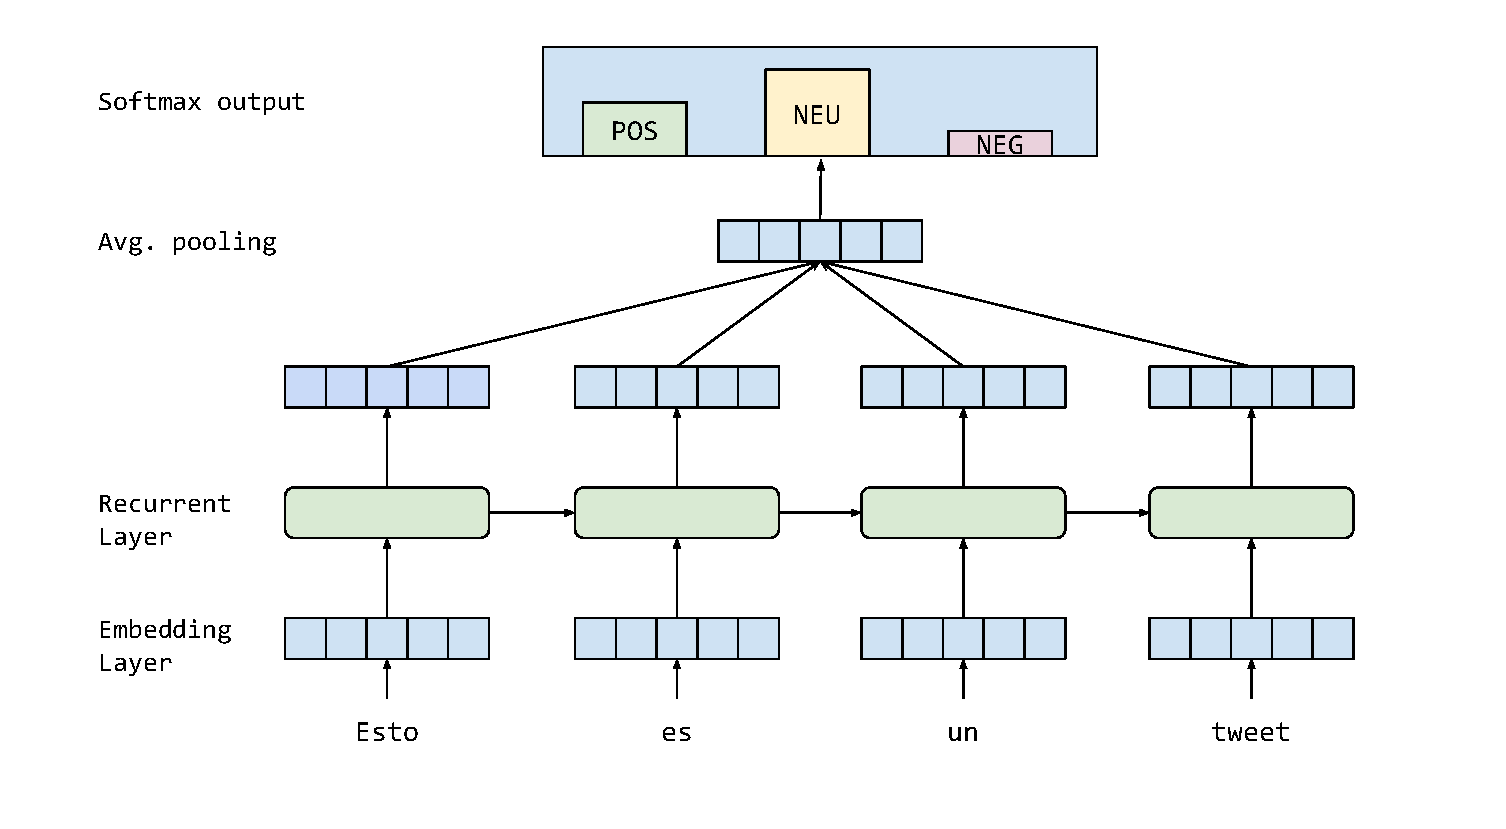
\includegraphics[width=\textwidth]{img/03/recurrent_classifier.pdf}
        \caption{Clasificador basado en redes recurrentes}
        \label{subfig:rnn_classifier}
    \end{subfigure}
    % Link a draw
    % https://docs.google.com/drawings/d/1KWz2NJGVoTO-pAAhhLjoX4AT-kSbK3yapLKLuQ2E9zw/edit
    \begin{subfigure}[t]{\textwidth}
        \centering
        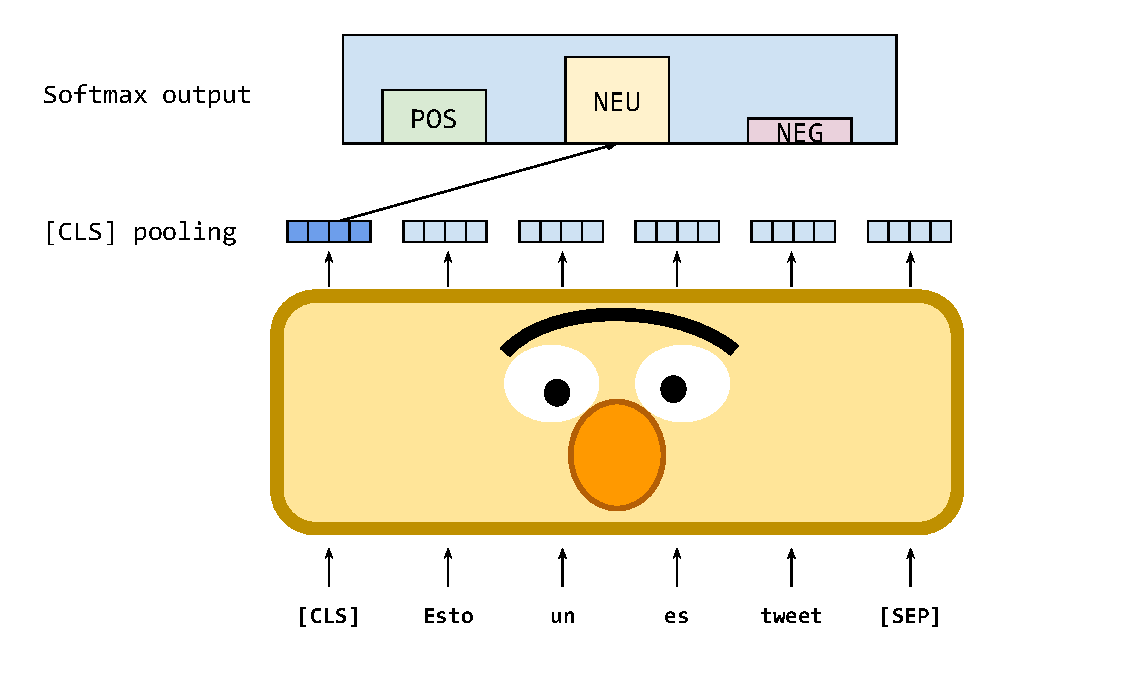
\includegraphics[width=\textwidth]{img/03/bert_classifier.pdf}
        \caption{Modelos de clasificación basado en BERT y símiles}
        \label{subfig:bert_classifier}
    \end{subfigure}

    \caption{Clasificadores propuestos para las tareas de Análisis de Polaridad, Análisis de Emociones y Detección de Ironía. La subfigura \ref{subfig:rnn_classifier} muestra la arquitectura del modelo recurrente, que usa una capa de embeddings basados en \emph{fasttext} y codifica el tweet como el promedio de las salidas de la capa recurrente. La subfigura \ref{subfig:bert_classifier} muestra un clasificador basado en BERT, donde tomamos la salida del token \emph{[CLS]} como la codificación del tweet. Ambos usan un decodificador softmax}
    \label{fig:03_classifiers}
\end{figure}

Describimos a continuación los clasificadores utilizados para las tareas. Podemos, a grandes rasgos, describir a todos nuestros clasificadores como compuestos de dos partes: un \emph{codificador} (o \emph{encoder} en inglés) que genera una representación contínua de longitud fija del texto de entrada, y un \emph{decodificador} que toma esa codificación y la convierte a la salida deseada.

Todos nuestros problemas analizados son de clasificación multiclase: elegir exactamente una clase entre varias. Para ello, nuestro decodificador será de la forma $\text{softmax}(Wx + b)$, donde $W$ es una matriz de pesos y $b$ un vector de bias, ambos parámetros de nuestra red neuronal.

Nuestros modelos diferirán entonces en los codificadores. Proponemos las siguientes variantes:

\begin{itemize}
    \item \textbf{FFN}: Un perceptrón multicapa (feed-forward network) con una función de activación intermedia \emph{ReLU}
    \item \textbf{GRU/biGRU}: Una red neuronal recurrente. La capa oculta es una Gated Recurrent Unit (GRU) unidireccional o bidireccional.
    \item \textbf{BETO|mBERT|RoBERTa|BERTin}: un modelo pre-entrenado de lenguaje basado en transformers.
\end{itemize}

En el caso de la \textbf{FFN}, la codificación se da luego de aplicar la función ReLU a la capa intermedia de la red. En el caso de la \textbf{GRU/biGRU}, la codificación se da como el promedio de los vectores salida de cada paso (podemos pensar cada uno de estos como representaciones contextualizadas de cada palabra). En el caso de los modelos basados en transformers, la codificación se da tomando la salida del caracter de inicio (\textbf{[CLS]} en el caso de BERT pero puede variar para RoBERTa u otros modelos)\footnote{Si bien podría también tomarse el promedio como en el caso de las redes recurrentes, los modelos basados en transformers no sufren el cuello de botella que se genera tomando la última representación de la red recurrente}. La figura \ref{fig:03_classifiers} ilustra la arquitectura de los clasificadores recurrentes y basados en transformers.

Usamos un tamaño oculto de 512 para los modelos recurrentes y FFN, y para todos los casos un dropout \cite{srivastava2014dropout} de 0.1 sobre la codificación del tweet. Para los dos primeros modelos, los entrenamos usando Adam con un learning rate de 0.001 con un decay de 0.01. Para los modelos basados en transformers, usamos Adam con un learning rate triangular de $10^{-5}$ y un warmup del 10\% de los pasos. Entrenamos todos los modelos por 5 epochs y nos quedamos con los modelos que mejor performance tengan sobre el split de validación en términos de la métrica correspondiente a la tarea.

\section{Resultados}

\begin{table*}[t]
    \centering
    \large
    \begin{tabular}{l ccc l}
        \toprule
        Modelo         &  Polaridad         & Emociones         &   Ironía        &  Puntaje \\
        \hline
        RoBERTa        &  $0.670 \pm 0.006$ &  $0.527 \pm 0.015$& $0.721 \pm 0.008$ &  0.665 \\
        BERTin         &  $0.666 \pm 0.005$ &  $0.524 \pm 0.007$& $0.713 \pm 0.012$ &  0.660 \\
        BETO$_U$       &  $0.651 \pm 0.006$ &  $0.532 \pm 0.012$& $0.701 \pm 0.007$ &  0.653 \\
        BETO$_C$       &  $0.662 \pm 0.005$ &  $0.516 \pm 0.012$& $0.705 \pm 0.009$ &  0.652 \\
        mBERT          &  $0.617 \pm 0.003$ &  $0.493 \pm 0.010$& $0.681 \pm 0.010$ &  0.627 \\
        \hline
        biGRU$_{TW}$   &  $0.585 \pm 0.011$ &  $0.264 \pm 0.007$& $0.631 \pm 0.011$ &  0.518 \\
        biGRU$_{CC}$   &  $0.553 \pm 0.008$ &  $0.231 \pm 0.006$& $0.625 \pm 0.009$ &  0.486 \\
        GRU$_{TW}$     &  $0.602 \pm 0.004$ &  $0.269 \pm 0.003$& $0.628 \pm 0.014$ &  0.509 \\
        GRU$_{CC}$     &  $0.564 \pm 0.004$ &  $0.237 \pm 0.005$& $0.581 \pm 0.016$ &  0.474 \\
        ffn$_{TW}$     &  $0.516 \pm 0.004$ &  $0.203 \pm 0.003$& $0.627 \pm 0.004$ &  0.433 \\
        ffn$_{CC}$     &  $0.509 \pm 0.003$ &  $0.179 \pm 0.001$& $0.481 \pm 0.003$ &  0.393 \\
        %robertuito     &  0.560 \pm 0.010 &  0.759 \pm 0.007 &  0.739 \pm 0.005 &  0.705 \pm 0.003 &  0.691 \\
        \hline
    \end{tabular}
    \caption{Resultados de la evaluación de los distintos modelos para las 3 tareas analizadas (Análisis de Emociones, Análisis de Emociones, Detección de Ironía). Los 3 resultados están dados en Macro F1, y expresados como la media de diez corridas junto a su desviación estándar. El puntaje de cada modelo es el promedio de las métricas para las 3 tareas}
    \label{tab:03_classification_results}
\end{table*}

La tabla \ref{tab:03_classification_results} muestra los resultados obtenidos con los distintos modelos de clasificación, expresados como la media de diez corridas de los experimentos de clasificación junto a sus desviaciones estándar; esto lo realizamos con motivo de que el entrenamiento es estocástico a diferencia de otros modelos clásicos de Machine Learning.Podemos observar que los mejores resultados se obtienen con el modelo \emph{roberta-bne} para las 3 tareas, aunque las diferencias son pequeñas. Todos los modelos basados en modelos pre-entrenados de transformers obtienen mejor performance que los basados en redes neuronales recurrentes.

Dentro de los modelos basados en redes recurrentes y feed-forward, aquellos que consumen embeddings entrenados en textos sociales (marcadas como $_{TW}$) obtienen mejor performance que aquellos que consumen embeddings entrenados en Common Crawl (marcados como $_{CC}$). Esta diferencia, en todos los casos, es estadísticamente significa corriendo un test U de Mann-Whitney ( $p \leq 0.05$ para el caso de ironía y \emph{biGRU}, para todas las demás comparaciones $p \leq 0.001$ ).




\section{Librería de análisis de sentimientos}

\newcommand{\pysentimiento}[0]{\textbf{pysentimiento}}

Algo que suele obstaculizar la utilización de herramientas de extracción de opinión (como las que acabamos de ver en este capítulo pero así mismo las que veremos más adelante) con fines de investigación es la dificultad a su acceso. O bien estos servicios están detrás de APIs pagas con precios demasiado altos para los presupuestos académicos o están disponibles pero no en español (u otro idioma de ``bajos recursos''). En otros casos, estos recursos están disponibles pero no para ser usados de forma de ``caja negra'', lo cual para alguien que no es un experto en NLP suele complicar su utilización.

Como una pequeñísima contribución de esta tesis y con el objetivo de facilitar el acceso de estos recursos para la investigación, creamos la librería \textbf{pysentimiento}\footnote{\url{https://github.com/pysentimiento/pysentimiento}}. Este paquete provee modelos pre-entrenados y herramientas de preprocesado para textos sociales. Si bien tiene soporte multilingual tanto en español como inglés, su eje original es el de proveer recursos para el español que tiene una disparidad importante en recursos.

La figura XXX muestra la arquitectura de \pysentimiento{}. Utiliza el model hub de \emph{huggingface}\footnote{\url{https://huggingface.co/models}}, un repositorio de modelos pre-entrenados basados en transformers. Allí es donde colocamos todos los modelos que entrenamos, tanto de sentimientos, emociones, y los que mostraremos más adelante como detección de discurso de odio. Cada tweet que es analizado por la librería pasa primero por una etapa de preprocesamiento (siguiendo el proceso explicado en la sección zzz), y luego procesado por el modelo, quien nos brinda un output. Dependiendo el problema, puede haber una etapa de post-procesamiento.

\todo{Completar las cosas que quedaron acá sin referencias}



%
% Pysentimiento architecture
% https://www.canva.com/design/DAEufPDskMI/Gg_phzjuXgFihF1g3x9L-A/edit#
%
%

\section{Discusión}

Para las 3 tareas planteadas, los clasificadores basados en modelos pre-entrenados de transformers obtuvieron mejores resultados que los basados en redes recurrentes y feed-forward. Como es esperable (y se observa en la literatura) los modelos monolinguales (\roberta{}, BERTin y \beto{}) tienen una performance sensiblemente mejor el modelo multilingual \emph{mBERT} \todo{citation needed de esto}. Dentro de los modelos de mejor performance, \roberta{} obtiene la mejor performance, aunque su mejora es pequeña respecto de \beto{}.

Algo que observamos es que, entre los modelos recurrentes y feed-forward que consumen word-embeddings, la utilización de representaciones entrenadas directamente sobre textos generados por usuario generan una mejor performance de los clasificadores. Si bien puede pensarse que el entorno pequeño o el texto ruidoso de los textos podrían ser un problema a la hora de construir representaciones

Retomaremos esta idea en el capítulo \ref{chap:07_domain_adaptation}, donde por un lado generaremos un modelo basado en RoBERTa entrenado sobre tweets, y por otro lado observaremos si podemos replicar su performance intentando ``adaptar'' un modelo \beto{} a este nuevo dominio.

Finalmente, como un pequeño aporte -- principalmente a la comunidad académica, y puntualmente aquella hispanoparlante -- creamos una librería de análisis de sentimientos \textbf{pysentimiento} que provee modelos pre-entrenados y herramientas de preprocesado para textos sociales. En esta herramienta quedarán volcados todos los modelos entrenados de esta tesis.

\section{Conclusiones}

En este capítulo hemos hecho una introducción a la extracción de opiniones usando técnicas de clasificación basadas en redes neuronales. Analizamos tres problemas de extracción de opiniones en Español --análisis de polaridad, análisis de emociones y detección de ironía-- y utilizamos modelos basados en redes neuronales y otros basados en modelos pre-entrenados. Presentamos el andamiaje básico para tareas de clasificación que utilizaremos en el resto de la presente tesis. En los siguientes capítulos centraremos nuestra atención en una tarea particular: la detección de discurso de odio.

\section{Notas}

Gran parte de este trabajo está basado en nuestra participación en TASS 2018\cite{overview_tass2018} resumida en \citet{atalaya_tass2018}. Los resultados en esta sección no son comparables con los de ese trabajo ya que decidimos utilizar la versión del dataset de TASS 2020\cite{garcia2020overview}, que por un lado unifica las dos posibles clases neutrales de TASS 2018 y además brinda el nuevo dataset de análisis de emociones. Omitimos el análisis de data augmentation y nos centramos en dar una breve introducción al tema y a analizar el impacto de los word-embeddings generados en textos sociales.
